\documentclass[preprint,review,12pt]{elsarticle}

\usepackage{amsmath,amssymb,amsfonts}
\usepackage{graphicx}
\usepackage{textcomp}
\usepackage{xcolor}
\usepackage{booktabs}
\usepackage{multirow}
\usepackage{url}
\usepackage{siunitx}
\usepackage{lineno}
\usepackage{hyperref}

% Compact lists
\usepackage{enumitem}
\setlist{nosep,leftmargin=*}

% Line numbers for review
\modulolinenumbers[5]

\journal{Journal of Systems Architecture}

\begin{document}

\begin{frontmatter}

\title{Predictive Modeling of Generative AI Inference Cost Across Hardware Architectures}

\author[ajou]{Yongjun Kim\corref{cor1}}
\ead{yjkim0123@ajou.ac.kr}
\cortext[cor1]{Corresponding author.}

\affiliation[ajou]{organization={Department of Software, Ajou University},
            city={Suwon},
            postcode={16499},
            country={Republic of Korea}}

\begin{abstract}
Deploying generative AI models across heterogeneous hardware requires accurate cost estimation at design time, yet inference energy and latency vary dramatically with model architecture, output configuration, and platform characteristics.
This paper presents a systematic framework for predicting generative AI inference cost from architectural and hardware parameters without executing the target workload.
Using \input{results/tex/n_raw_records.tex}\unskip{} energy measurements spanning \input{results/tex/n_models.tex}\unskip{} generative models (autoregressive and diffusion-based) across three hardware platforms (Apple M4~Pro, NVIDIA A100, NVIDIA H100), individual measurements from \input{results/tex/n_configs.tex}\unskip{} unique configurations (${\sim}$\input{results/tex/mean_reps.tex}\unskip{} repetitions each) are used to train and evaluate five regression methods under three cross-validation strategies: standard $k$-fold, leave-one-hardware-out~(LOHO), and leave-one-model-out~(LOMO).
SVR with log-transformed features achieves $R^2 {=}$\,\input{results/tex/kfold_best_r2.tex}\unskip{} and MAPE of \input{results/tex/kfold_best_mape.tex}\unskip\% under $k$-fold CV, demonstrating that accurate cost prediction is feasible when the target hardware is known.
However, LOHO-CV reveals a fundamental generalization gap: predicting energy on entirely unseen hardware degrades to $R^2 {<} 0.1$, exposing the limits of black-box models for cross-platform extrapolation.
SHAP analysis uncovers architecture-dependent cost drivers: hardware thermal design power dominates for autoregressive models (mean $|\text{SHAP}| {=}$\,\input{results/tex/shap_ar_tdp.tex}\unskip), while output complexity and diffusion steps dominate for diffusion models.
These findings provide system designers and practitioners with actionable guidance for hardware-aware inference cost estimation and workload-to-platform mapping.
\end{abstract}

\begin{keyword}
Energy modeling \sep Generative AI \sep Inference cost prediction \sep Hardware-aware design \sep Cross-platform estimation \sep SHAP analysis
\end{keyword}

\end{frontmatter}

\linenumbers

%======================================================================
\section{Introduction}
\label{sec:introduction}
%======================================================================

The proliferation of generative AI---spanning large language models~(LLMs), image diffusion models, video generators, and audio synthesizers---has created an urgent need for hardware-aware inference cost modeling.
Data center operators, edge device designers, and system architects must estimate energy consumption and latency \emph{before} committing to specific hardware, yet the design space of models, configurations, and platforms is vast.
The rapid pace of model releases---with new architectures appearing monthly---exacerbates this problem, as exhaustive profiling of every model--hardware combination is infeasible.

The environmental and economic stakes are substantial.
Recent estimates suggest that AI workloads already account for a significant and growing fraction of global data center energy consumption~\cite{patterson2021carbon,wu2022sustainable}, with inference---rather than training---constituting the majority of operational cost for deployed models~\cite{desislavov2023trends}.
The International Energy Agency projects that data center electricity demand could more than double by 2026, driven in part by AI workloads~\cite{iea2024electricity}.
This concern has catalyzed the ``Green AI'' movement~\cite{schwartz2020green}, which advocates for energy efficiency as a first-class evaluation metric alongside accuracy and throughput.
Accurate inference cost modeling is a prerequisite for this agenda: one cannot optimize what one cannot predict.

The challenge extends beyond data centers.
Edge deployment of generative AI---on mobile devices, embedded systems, and on-premise servers---introduces additional constraints where power budgets are tight and thermal envelopes are limited~\cite{xu2024survey_edge}.
A model that consumes \SI{50}{\joule} per inference on an NVIDIA H100 may consume \SI{5}{\joule} on an Apple M4~Pro, but the latency and user experience implications differ qualitatively.
System architects need predictive tools that can estimate these tradeoffs from model and hardware specifications alone, without requiring access to every target platform.

Two fundamental architectural paradigms dominate generative AI: \emph{autoregressive}~(AR) models that generate tokens sequentially, and \emph{diffusion} models that iteratively denoise through multiple steps.
These paradigms exhibit fundamentally different computational profiles---AR cost scales with output token count while diffusion cost scales with the product of spatial resolution and step count---making unified cost prediction challenging.
Moreover, the hardware landscape is increasingly heterogeneous: NVIDIA datacenter GPUs (A100, H100), Apple Silicon SoCs with unified memory, Google TPUs, AMD Instinct accelerators, and various NPUs each offer different performance--power tradeoffs~\cite{jouppi2017datacenter}.
A cost model that works within one hardware family may fail entirely when extrapolating to a different architecture class.

This paper addresses the question: \emph{Can generative AI inference cost be predicted from model and hardware parameters alone, without running the workload on the target platform?}
To answer this, we construct a dataset of \input{results/tex/n_raw_records.tex}\unskip{} energy measurements spanning seven generative models across three hardware platforms, train five regression methods under three cross-validation strategies of increasing difficulty, and apply SHAP analysis to identify architecture-dependent cost drivers.

The contributions of this work are:
\begin{enumerate}
\item A unified dataset of \input{results/tex/n_raw_records.tex}\unskip{} energy and latency measurements across seven generative models, four modalities (text, image, video, music) with varying batch configurations, and three hardware platforms spanning a 17.5$\times$ range in TDP.
\item A systematic comparison of five regression methods under three cross-validation strategies, revealing a fundamental generalization gap between within-platform prediction ($R^2 {>} 0.9$) and cross-platform extrapolation ($R^2 {<} 0.1$).
\item SHAP-based analysis showing that the dominant cost drivers differ fundamentally between AR and diffusion architectures---AR inference is hardware-bound (TDP dominates) while diffusion inference is workload-bound (output complexity and step count dominate)---providing actionable insights for system designers.
\item An analytical log-linear cost formula and practical guidelines for hardware-aware cost estimation at design time, with implications for SoC power budgeting and hardware design space exploration.
\end{enumerate}

The remainder of this paper is organized as follows.
Section~\ref{sec:related_work} reviews related work on neural network cost modeling, generative AI energy profiling, and cross-platform performance prediction.
Section~\ref{sec:methodology} describes the measurement infrastructure, dataset, feature engineering, regression methods, cross-validation strategies, evaluation metrics, and SHAP analysis methodology.
Section~\ref{sec:results} presents the experimental results under all three evaluation protocols.
Section~\ref{sec:discussion} discusses the generalization gap, systems implications, practical guidelines, limitations, and threats to validity.
Section~\ref{sec:conclusion} concludes with future research directions.


%======================================================================
\section{Related Work}
\label{sec:related_work}
%======================================================================

This section reviews three bodies of literature that motivate and contextualize our work: neural network cost modeling, generative AI energy profiling, and cross-platform performance prediction.

%----------------------------------------------------------------------
\subsection{Neural Network Cost Modeling}
\label{sec:rw_cost_modeling}
%----------------------------------------------------------------------

System-level energy modeling has a long history in the computer systems communities.
Wattch~\cite{brooks2000wattch} pioneered microarchitectural power estimation by decomposing processor energy into functional unit contributions, enabling architects to evaluate design tradeoffs without fabrication.
DRAMPower~\cite{chandrasekar2012drampower} extended power modeling to memory subsystems, and Accelergy~\cite{wu2019machine} provided an architecture-level methodology for estimating energy in custom accelerator designs.
These tools operate at the microarchitectural level, requiring detailed knowledge of the hardware design---information that is typically unavailable for commercial platforms.

For neural network workloads specifically, several cost models have been proposed.
Yang et al.~\cite{yang2017designing} developed energy-aware pruning by modeling per-layer energy as a function of operation counts and data movement.
NeuralPower~\cite{cai2017neuralpower} predicts CNN inference power from layer-wise architectural features using polynomial regression.
Eyeriss~\cite{chen2016eyeriss} introduced an energy-efficient dataflow for CNNs and provided an analytical framework for estimating energy based on data reuse patterns.
More recently, nn-Meter~\cite{zhang2021nnmeter} predicts latency on diverse edge devices by decomposing neural architectures into kernel-level primitives and profiling each kernel type, achieving high accuracy within specific device families.

These approaches share a common limitation: they focus on classification or recognition workloads with fixed-size inputs and outputs.
Generative models introduce variable-length outputs---a 32-token text completion and a 512-token response differ by 16$\times$ in computational cost---which existing frameworks do not address.
Furthermore, most neural network cost models target a single hardware platform or a narrow class of accelerators, leaving the cross-platform prediction problem unexplored.

The roofline model~\cite{williams2009roofline} provides hardware-centric performance bounds based on arithmetic intensity and peak hardware capabilities.
While insightful for understanding computational bottlenecks, the roofline model assumes well-characterized workloads and does not directly predict energy consumption across diverse generative AI configurations.
Our work complements these microarchitectural and analytical approaches by operating at the \emph{system level}, using only high-level model and hardware specifications available from datasheets.

%----------------------------------------------------------------------
\subsection{LLM and Generative AI Energy Profiling}
\label{sec:rw_energy_profiling}
%----------------------------------------------------------------------

The energy cost of large-scale AI has received increasing attention.
Patterson et al.~\cite{patterson2021carbon} estimated the carbon footprint of training large models, finding that training a single large model can emit as much carbon as five automobiles over their lifetimes.
Wu et al.~\cite{wu2022sustainable} analyzed the environmental implications of AI across the full lifecycle, including both training and inference.
Strubell et al.~\cite{strubell2019energy} provided early estimates of the energy and policy considerations of NLP model training, catalyzing broader awareness.
However, these studies focus primarily on \emph{training} costs, whereas \emph{inference} dominates the operational energy budget of deployed models~\cite{desislavov2023trends}.

Several recent studies have begun to characterize inference energy specifically.
Samsi et al.~\cite{samsi2023words} benchmarked the energy cost of LLM inference (``From Words to Watts''), measuring multiple models on NVIDIA GPUs and reporting per-token energy costs.
Chien et al.~\cite{chien2023reducing} projected the carbon impact of generative AI inference to 2035 under various scaling scenarios.
Luccioni et al.~\cite{luccioni2024power} conducted a multi-model, multi-task energy audit (``Power Hungry Processing''), measuring 88 models across inference tasks and finding that generative tasks consume substantially more energy than discriminative ones.
Dodge et al.~\cite{dodge2022measuring} proposed standardized methodologies for measuring the carbon intensity of AI systems, including recommendations for reporting inference costs.

For diffusion models specifically, energy consumption scales with the number of denoising steps, spatial resolution, and guidance scale.
Rombach et al.~\cite{rombach2022high} introduced latent diffusion to reduce computational cost by operating in a compressed latent space, and subsequent work on progressive distillation~\cite{salimans2022progressive} and consistency models~\cite{song2023consistency} has sought to reduce the number of required steps.
These algorithmic advances directly affect inference energy, yet their impact has not been systematically modeled as a function of hardware characteristics.

Critically, all of the above studies \emph{report} measured energy costs for specific model--hardware combinations rather than \emph{predicting} costs for unseen configurations.
They provide valuable empirical data but do not construct predictive models.
Our work bridges this gap by building regression models that estimate inference energy from model and hardware parameters alone.

%----------------------------------------------------------------------
\subsection{Cross-Platform Performance Prediction}
\label{sec:rw_cross_platform}
%----------------------------------------------------------------------

Predicting performance across different hardware platforms is a longstanding challenge in computer architecture.
Lee et al.~\cite{lee2006accurate} developed cross-platform performance prediction using statistical models trained on hardware performance counters, demonstrating that workload behavior on one microarchitecture can partially predict behavior on another.
Ardalani et al.~\cite{ardalani2015cross} extended this to GPU workloads, using static code features and machine learning to predict GPU execution time from CPU execution characteristics.
Rethinagiri et al.~\cite{rethinagiri2014system} proposed a system-level power estimation tool for embedded platforms using abstract workload signatures.

In the machine learning domain, hardware-aware neural architecture search (NAS) has driven interest in latency and energy prediction across devices.
nn-Meter~\cite{zhang2021nnmeter} achieves accurate latency prediction within device families by building device-specific kernel latency predictors.
BRP-NAS~\cite{dudziak2020brpnas} uses predictor-based NAS with hardware-aware objectives, training surrogate models on a few hundred architecture evaluations per device.
HELP~\cite{lee2021help} addresses cross-device latency prediction through hardware-adaptive transfer, using a small number of measurements on the target device to calibrate a model trained on source devices.
These works demonstrate that hardware-specific calibration is essential for cross-platform prediction---a finding our results strongly corroborate.

Transfer learning and domain adaptation approaches have shown promise for bridging platform gaps.
Kaufman et al.~\cite{kaufman2021learned} proposed learned performance models for TPU design space exploration, training models on simulation data and transferring to real hardware.
However, these techniques typically require at least a small set of measurements on the target platform, and their applicability to generative AI workloads---with variable-length outputs and diverse modalities---remains unexplored.

The use of SHAP (SHapley Additive exPlanations)~\cite{lundberg2017shap} for interpretable power modeling has been explored by Zhang et al.~\cite{zhang2020shap}, who applied SHAP to multicore processor power models to identify dominant performance counters.
Our work extends SHAP analysis to generative AI cost models, revealing architecture-dependent (AR vs.\ diffusion) cost driver patterns that have not been previously documented.

%----------------------------------------------------------------------
\subsection{Positioning of This Work}
\label{sec:rw_positioning}
%----------------------------------------------------------------------

Table~\ref{tab:related_comparison} summarizes the positioning of this work relative to existing literature.
Several gaps in the literature motivate our contribution.
First, existing neural network cost models focus on classification workloads with fixed-size inputs/outputs, whereas generative models exhibit order-of-magnitude variation in output complexity.
Second, energy profiling studies for LLMs and diffusion models report measured costs but do not construct predictive models.
Third, cross-platform prediction has been studied for general compute workloads and NAS latency but not for generative AI energy.
Fourth, no prior work has systematically compared within-platform and cross-platform prediction accuracy for inference energy, nor identified the architecture-dependent cost driver dichotomy (hardware-bound AR vs.\ workload-bound diffusion) via SHAP analysis.

This study addresses all four gaps by combining a multi-model, multi-platform measurement dataset with systematic cross-validation evaluation and interpretable feature importance analysis.
The cost model operates at the system level---complementing microarchitectural tools with rapid design-time estimates---and the SHAP-based decomposition provides actionable guidance for both hardware designers and model developers.

\begin{table}[t]
\centering
\caption{Comparison with Related Work}
\label{tab:related_comparison}
\footnotesize
\begin{tabular}{@{}p{2.8cm}cccc@{}}
\toprule
\textbf{Study} & \textbf{GenAI} & \textbf{Predict} & \textbf{Cross-HW} & \textbf{Interp.} \\
\midrule
Wattch~\cite{brooks2000wattch} & -- & \checkmark & -- & -- \\
NeuralPower~\cite{cai2017neuralpower} & -- & \checkmark & -- & -- \\
nn-Meter~\cite{zhang2021nnmeter} & -- & \checkmark & partial & -- \\
Samsi et al.~\cite{samsi2023words} & \checkmark & -- & -- & -- \\
Luccioni et al.~\cite{luccioni2024power} & \checkmark & -- & -- & -- \\
Dodge et al.~\cite{dodge2022measuring} & -- & -- & -- & -- \\
HELP~\cite{lee2021help} & -- & \checkmark & \checkmark & -- \\
\textbf{This work} & \checkmark & \checkmark & \checkmark & \checkmark \\
\bottomrule
\end{tabular}
\vspace{1mm}
\raggedright\scriptsize
GenAI: covers generative AI workloads; Predict: builds predictive models (not just reporting measurements); Cross-HW: evaluates cross-hardware generalization; Interp.: provides interpretable feature importance (SHAP).
\end{table}


%======================================================================
\section{Methodology}
\label{sec:methodology}
%======================================================================

\subsection{Measurement Infrastructure}
\label{sec:measurement}
Inference energy measurements were collected using platform-specific instrumentation:
NVIDIA GPUs via \texttt{nvidia-smi} power sampling at \SI{100}{\milli\second} intervals,
and Apple M4~Pro via \texttt{powermetrics} at \SI{500}{\milli\second} resolution.
Each configuration was repeated approximately 30 times to capture run-to-run variance.
The \input{results/tex/n_raw_records.tex}\unskip{} individual measurements are aggregated to \input{results/tex/n_configs.tex}\unskip{} configuration-level means (${\sim}$\input{results/tex/mean_reps.tex}\unskip{} repetitions each) prior to modeling, ensuring no data leakage across CV folds.

For NVIDIA GPUs, energy is computed by integrating instantaneous power readings over the inference duration: $E = \sum_{t} P(t) \cdot \Delta t$, where $P(t)$ is the GPU power draw at time $t$ and $\Delta t = \SI{100}{\milli\second}$ is the sampling interval.
For the Apple M4~Pro, \texttt{powermetrics} reports package-level power consumption including CPU, GPU, and memory subsystems.
While the instrumentation granularity differs across platforms, both approaches capture the total system-level energy attributable to the inference workload.
Warm-up runs were conducted before measurement to ensure steady-state thermal conditions, and idle power was not subtracted, as our goal is to model total system energy during inference---the quantity relevant for operational cost estimation.

\subsection{Models, Hardware, and Configurations}
\label{sec:models_hw}
Table~\ref{tab:models_hw} summarizes the seven generative models and three hardware platforms.
The dataset spans four modalities (text, image, video, music) with varying batch configurations: token counts from 32 to 512, image resolutions from $128{\times}128$ to $640{\times}640$, video frame counts from 4 to 16, diffusion steps from 5 to 50, and batch sizes from 1 to 16.
The dataset comprises \input{results/tex/n_raw_records.tex}\unskip{} individual measurements across \input{results/tex/n_configs.tex}\unskip{} unique configurations (${\sim}$\input{results/tex/mean_reps.tex}\unskip{} repetitions per configuration), with energy ranging from \SI{3.1}{\joule} to \SI{1728}{\joule} and latency from \SI{0.16}{\second} to \SI{71}{\second}.

The models were selected to represent the two dominant generative paradigms (autoregressive and diffusion) across diverse modalities.
Phi-3-mini-4k and Mistral-7B represent autoregressive text generation at different scales.
MusicGen-small and MusicGen-medium represent autoregressive audio generation.
Stable Diffusion v1.5, SDXL-base-1.0, and AnimateDiff-v1.5 represent diffusion-based image and video generation.
This selection covers a range of model sizes (0.6B to 7.2B parameters) and output modalities.

The three hardware platforms were chosen to span a wide range of compute capabilities and power envelopes: from a 40\,W unified-memory SoC (Apple M4~Pro) to a 700\,W datacenter GPU (NVIDIA H100).
This 17.5$\times$ TDP range and the qualitative difference between unified-memory and discrete-GPU architectures create a challenging testbed for cross-platform prediction.

Not all models were tested on all platforms, as shown in the coverage matrix (Table~\ref{tab:coverage}).
Mistral-7B was measured only on the A100 due to memory constraints on the M4~Pro and availability on the H100.
MusicGen variants were tested on M4~Pro and A100 but not H100.
This incomplete coverage reflects practical deployment realities and is accounted for in the cross-validation analysis.

\begin{table}[t]
\centering
\caption{Models, Hardware Platforms, and Coverage}
\label{tab:models_hw}
\footnotesize
\begin{tabular}{@{}llrlccc@{}}
\toprule
\textbf{Model} & \textbf{Type} & \textbf{Params} & \textbf{Mod.} & \textbf{M4P} & \textbf{A100} & \textbf{H100} \\
\midrule
Phi-3-mini-4k      & AR   & 3.8\,B  & Text  & \checkmark & \checkmark & \checkmark \\
Mistral-7B         & AR   & 7.2\,B  & Text  & -- & \checkmark & -- \\
MusicGen-small     & AR   & 0.6\,B  & Music & \checkmark & \checkmark & -- \\
MusicGen-medium    & AR   & 1.5\,B  & Music & \checkmark & \checkmark & -- \\
SD-v1-5            & Diff & 0.9\,B  & Image & \checkmark & \checkmark & \checkmark \\
SDXL-base-1.0      & Diff & 3.5\,B  & Image & \checkmark & \checkmark & \checkmark \\
AnimateDiff-v1.5   & Diff & 0.9\,B  & Video & \checkmark & \checkmark & \checkmark \\
\midrule
\textbf{Hardware} & \textbf{TDP} & \textbf{Mem.\,BW} & \multicolumn{4}{l}{\textbf{Compute}} \\
\midrule
Apple M4 Pro     & 40\,W  & 273\,GB/s  & \multicolumn{4}{l}{20 GPU cores} \\
NVIDIA A100 40GB & 400\,W & 1555\,GB/s & \multicolumn{4}{l}{6912 CUDA cores} \\
NVIDIA H100 80GB & 700\,W & 3350\,GB/s & \multicolumn{4}{l}{14592 CUDA cores} \\
\bottomrule
\end{tabular}
\vspace{1mm}
\raggedright\scriptsize
Checkmarks indicate measured combinations. Not all models were tested on all platforms; Mistral-7B was measured only on A100, and MusicGen variants only on M4~Pro and A100. This affects LOHO and LOMO evaluation as discussed in the text.
\end{table}

\begin{table}[t]
\centering
\caption{Model--Platform Coverage Matrix}
\label{tab:coverage}
\footnotesize
\begin{tabular}{@{}lccc@{}}
\toprule
\textbf{Model} & \textbf{M4 Pro} & \textbf{A100} & \textbf{H100} \\
\midrule
AnimateDiff-v1.5 & \checkmark & \checkmark & \checkmark \\
Mistral-7B-Instruct & -- & \checkmark & -- \\
MusicGen-medium & \checkmark & \checkmark & -- \\
MusicGen-small & \checkmark & \checkmark & -- \\
Phi-3-mini-4k & \checkmark & \checkmark & \checkmark \\
SD-v1-5 & \checkmark & \checkmark & \checkmark \\
SDXL-base-1.0 & \checkmark & \checkmark & \checkmark \\
\bottomrule
\end{tabular}
\end{table}

\subsection{Feature Engineering}
\label{sec:features}
Eight input features are engineered from model specifications and hardware datasheets, requiring \emph{no runtime profiling}:
\begin{itemize}
\item \textbf{Model:} parameter count (billions), architecture type (AR\,$=$\,0, Diffusion\,$=$\,1)
\item \textbf{Hardware:} thermal design power~(TDP, watts), compute units (GPU cores or CUDA cores), memory bandwidth~(GB/s)
\item \textbf{Configuration:} output complexity (tokens for text/music, pixels for images, pixel$\times$frames for video), diffusion steps (1 for AR), batch size
\end{itemize}
Output complexity provides a unified scalar that captures the workload magnitude across heterogeneous modalities.
All continuous features are log-transformed via $\log(1+x)$ to handle the multi-scale ranges (TDP: 40--700\,W; compute: 20--14592 units; energy: 3--1728\,J).
Target energy is also log-transformed for training; predictions are inverse-transformed before evaluation.

The choice of features reflects a deliberate design decision: we restrict to information available from published specifications and datasheets, without requiring any runtime measurement on the target hardware.
This enables \emph{design-time} cost estimation---the primary use case for system architects evaluating hardware procurement or workload placement decisions.

\subsection{Regression Methods}
\label{sec:regression}
Five regression approaches spanning parametric, kernel, and ensemble methods are evaluated:
Linear Regression, Ridge ($\alpha{=}1$), Random Forest (200 trees, max depth~12), XGBoost (200 boosters, max depth~8, learning rate~0.1), and SVR (RBF kernel, $C{=}100$).
For SVR, features are standardized; tree-based models operate on log-transformed features directly.
Hyperparameters were set to commonly used defaults from the scikit-learn and XGBoost documentation; no hyperparameter tuning was performed on the evaluation data.

The selection of methods is deliberate.
Linear Regression and Ridge represent the simplest parametric baselines and can reveal whether the log-transformed feature space admits a linear cost model.
Random Forest and XGBoost represent state-of-the-art tree-based ensembles that can capture nonlinear interactions.
SVR with an RBF kernel provides a kernel-based alternative that operates in a high-dimensional implicit feature space.
By comparing these approaches under identical cross-validation protocols, we can disentangle the effect of model complexity from the inherent difficulty of the prediction task.

\subsection{Cross-Validation Strategies}
\label{sec:cv}
Three CV strategies of increasing difficulty are employed:
\begin{enumerate}
\item \textbf{5-Fold CV:} random splits across all configurations; tests interpolation within the training distribution.
\item \textbf{Leave-One-Hardware-Out (LOHO):} train on two platforms, predict the third; tests cross-platform extrapolation---the key experiment for practical deployment.
\item \textbf{Leave-One-Model-Out (LOMO):} train on six models, predict the seventh; tests generalization to unseen architectures.
\end{enumerate}

LOHO simulates the realistic scenario where a designer wants to estimate inference cost on hardware that has not yet been profiled.
This is the most demanding test and the primary experiment of this work.
LOMO tests a complementary scenario: estimating the cost of a newly released model on already-profiled hardware.
Together, these three protocols provide a comprehensive picture of model generalization across different axes of variation.

\subsection{Evaluation Metrics}
\label{sec:metrics}
Three standard regression metrics are used to evaluate prediction quality:

\textbf{Coefficient of Determination ($R^2$):}
\begin{equation}
R^2 = 1 - \frac{\sum_{i=1}^{n}(y_i - \hat{y}_i)^2}{\sum_{i=1}^{n}(y_i - \bar{y})^2}
\label{eq:r2}
\end{equation}
where $y_i$ is the measured energy, $\hat{y}_i$ is the predicted energy, and $\bar{y}$ is the mean measured energy.
$R^2 = 1$ indicates perfect prediction; $R^2 = 0$ indicates that the model is no better than predicting the mean; negative values indicate that the model is worse than the mean predictor.
Negative $R^2$ values can occur under LOHO and LOMO when the training distribution differs substantially from the test distribution.

\textbf{Root Mean Squared Error (RMSE):}
\begin{equation}
\text{RMSE} = \sqrt{\frac{1}{n}\sum_{i=1}^{n}(y_i - \hat{y}_i)^2}
\label{eq:rmse}
\end{equation}
RMSE is reported in joules and provides an absolute measure of prediction error in the original energy units.

\textbf{Mean Absolute Percentage Error (MAPE):}
\begin{equation}
\text{MAPE} = \frac{100}{n}\sum_{i=1}^{n}\frac{|y_i - \hat{y}_i|}{y_i}
\label{eq:mape}
\end{equation}
MAPE provides a scale-independent error measure, enabling comparison across configurations with different energy magnitudes.
Given the wide energy range in our dataset (\SI{3.1}{\joule} to \SI{1728}{\joule}), MAPE is particularly informative as it weights errors proportionally to the true value.

All metrics are computed on the original (non-log) energy scale after inverse-transforming predictions, ensuring that reported errors reflect the quantities relevant to practitioners.

\subsection{SHAP Analysis}
\label{sec:shap_method}
To identify the dominant cost drivers and understand how they differ between architectural paradigms, we apply SHAP (SHapley Additive exPlanations)~\cite{lundberg2017shap} to the best-performing model (SVR under 5-fold CV).

SHAP values are rooted in cooperative game theory: for each prediction, the contribution of each feature is computed as the average marginal contribution across all possible feature coalitions.
Formally, the SHAP value $\phi_j$ for feature $j$ is:
\begin{equation}
\phi_j = \sum_{S \subseteq F \setminus \{j\}} \frac{|S|!\,(|F|-|S|-1)!}{|F|!} \left[ f(S \cup \{j\}) - f(S) \right]
\label{eq:shap}
\end{equation}
where $F$ is the full feature set, $S$ is a subset excluding feature $j$, and $f(S)$ is the model prediction using only features in $S$.
The key property of SHAP values is \emph{local accuracy}: the sum of all feature contributions plus the base value exactly equals the model prediction for each instance.

We compute SHAP values for all configurations and then decompose the analysis by architecture type (AR vs.\ diffusion) to reveal paradigm-specific cost drivers.
The mean absolute SHAP value $\overline{|\phi_j|}$ across instances provides a global importance ranking, while the distribution of SHAP values reveals the direction and magnitude of each feature's influence.
This decomposition is central to our finding that AR inference is hardware-bound while diffusion inference is workload-bound.


%======================================================================
\section{Results and Analysis}
\label{sec:results}
%======================================================================

\subsection{Within-Platform Prediction (5-Fold CV)}
\label{sec:results_kfold}

Table~\ref{tab:kfold} reports 5-fold CV results.
SVR achieves $R^2 {=}$\,\input{results/tex/kfold_best_r2.tex}\unskip{} with MAPE of \input{results/tex/kfold_best_mape.tex}\unskip\%, while linear models perform moderately ($R^2 {\approx} 0.57$) and tree-based ensembles achieve $0.76$--$0.84$.
The log transformation is critical: raw-feature models achieve substantially lower accuracy, confirming the multiplicative nature of the inference cost function.
When the target hardware is represented in training data, accurate prediction is feasible with simple features and standard regression methods.

The strong performance of SVR suggests that the RBF kernel captures nonlinear interactions between features that linear and tree-based models miss.
The moderate performance of linear models ($R^2 {\approx} 0.57$) indicates that while the log-transformed feature space is approximately linear, significant nonlinearities remain---likely arising from interactions between hardware capability and workload characteristics.

\begin{table}[t]
\centering
\caption{5-Fold Cross-Validation Results (Energy)}
\label{tab:kfold}
\footnotesize
\begin{tabular}{@{}lrrr@{}}
\toprule
\textbf{Method} & \textbf{R\textsuperscript{2}} & \textbf{RMSE (J)} & \textbf{MAPE (\%)} \\
\midrule
Linear & 0.571 & 243.8 & 45.1 \\
Ridge & 0.374 & 294.5 & 67.7 \\
RF & 0.761 & 182.1 & 36.8 \\
XGBoost & 0.839 & 149.4 & 34.1 \\
SVR & \textbf{0.923} & 103.3 & 14.2 \\
\bottomrule
\end{tabular}
\end{table}

\subsection{Cross-Platform Prediction (LOHO-CV)}
\label{sec:results_loho}

Table~\ref{tab:loho} presents the critical LOHO-CV results.
All models suffer dramatic performance degradation when predicting on unseen hardware.
Even the best performer (RF) achieves only $R^2 {=}$\,\input{results/tex/loho_best_r2.tex}\unskip{} overall.
This exposes a fundamental \emph{generalization gap}: models that achieve over 90\% accuracy within known platforms fail when extrapolating to new hardware.

\begin{table}[t]
\centering
\caption{Leave-One-Hardware-Out CV Results (Energy)}
\label{tab:loho}
\footnotesize
\begin{tabular}{@{}lrrr@{}}
\toprule
\textbf{Method} & \textbf{R\textsuperscript{2}} & \textbf{RMSE (J)} & \textbf{MAPE (\%)} \\
\midrule
Linear & -0.59 & 469.2 & 333.8 \\
Ridge & -0.80 & 499.5 & 397.4 \\
RF & 0.05 & 362.2 & 208.7 \\
XGBoost & -0.02 & 375.2 & 143.9 \\
SVR & -0.28 & 421.0 & 392.0 \\
\bottomrule
\end{tabular}
\end{table}

The per-platform breakdown (Table~\ref{tab:loho_hw}) reveals pronounced asymmetry.
The A100 is most predictable when held out (best MAPE of \input{results/tex/loho_a100_mape.tex}\unskip\%), as its specifications fall between the M4~Pro and H100, enabling interpolation.
The M4~Pro is hardest to predict (MAPE $>$\,375\% for all models), likely because its unified memory architecture and low TDP (\SI{40}{\watt} vs.\ \SI{400}{\watt}--\SI{700}{\watt} for GPUs) create a qualitatively different energy profile from discrete GPUs---models trained on high-TDP platforms systematically overestimate M4~Pro consumption.

\begin{table}[t]
\centering
\caption{Per-Platform LOHO Energy MAPE (\%)}
\label{tab:loho_hw}
\footnotesize
\begin{tabular}{@{}lrrr@{}}
\toprule
\textbf{Method} & \textbf{M4 Pro} & \textbf{A100} & \textbf{H100} \\
\midrule
Linear & 919.0 & 33.5 & 263.2 \\
Ridge & 993.1 & 33.5 & 352.8 \\
RF & 425.6 & 40.0 & 209.3 \\
XGBoost & 375.8 & 58.4 & 100.3 \\
SVR & 1077.0 & 40.1 & 309.5 \\
\bottomrule
\end{tabular}
\end{table}

Fig.~\ref{fig:loho_scatter} visualizes the LOHO predictions using XGBoost trained in log-transformed feature space.
Predictions cluster near the diagonal for A100 (interpolation regime) but show systematic bias for M4~Pro (extrapolation regime), confirming that the gap is structural rather than stochastic.

\begin{figure}[t]
\centering
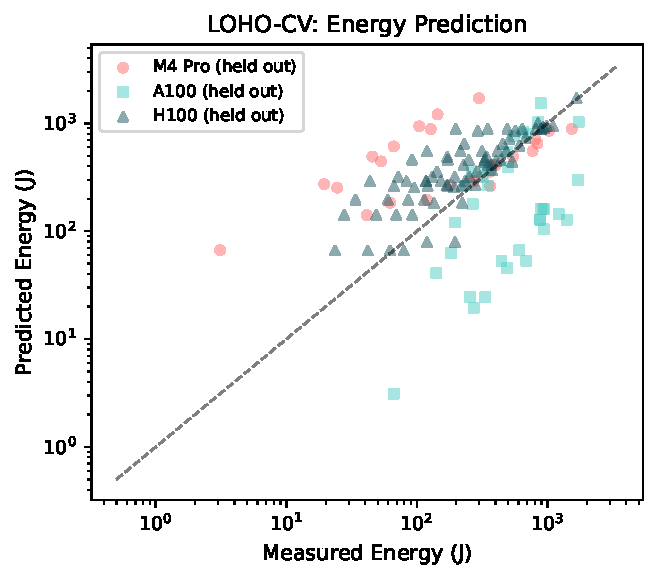
\includegraphics[width=\columnwidth]{figures/loho_scatter.pdf}
\caption{LOHO-CV predicted vs.\ measured inference energy using XGBoost in log-feature space. Each hardware platform is predicted by a model trained exclusively on the other two. A100 predictions (interpolation) closely follow the diagonal; M4~Pro predictions (extrapolation) show systematic overestimation.}
\label{fig:loho_scatter}
\end{figure}

Fig.~\ref{fig:loho_per_hw} further decomposes the LOHO error by held-out platform and regression method.
The per-platform MAPE reveals that M4~Pro prediction is catastrophically poor across all methods, with some log-space linear models exceeding 6,000\% MAPE.
In contrast, A100 MAPE remains below 100\% for most methods, confirming that interpolation between the M4~Pro and H100 is far more tractable than extrapolation beyond the training distribution.
Notably, tree-based methods (XGBoost, RF) degrade more gracefully than linear models under distribution shift, as they are less susceptible to extrapolation artifacts in log-space.

\begin{figure}[t]
\centering
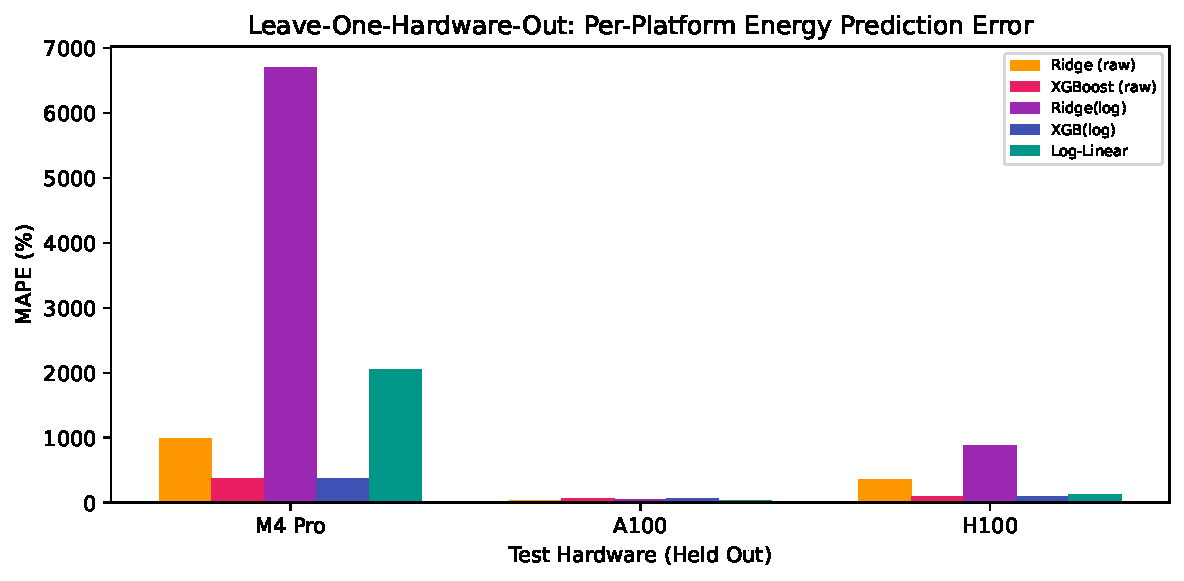
\includegraphics[width=\columnwidth]{figures/loho_per_hardware.pdf}
\caption{Per-platform LOHO energy prediction error (MAPE) for each regression method. M4~Pro (held out) yields catastrophic errors across all methods; A100 (held out) is well-predicted via interpolation; H100 shows intermediate difficulty. Log-space linear models are particularly unstable for M4~Pro.}
\label{fig:loho_per_hw}
\end{figure}

\subsection{Cross-Model Prediction (LOMO-CV)}
\label{sec:results_lomo}

LOMO-CV evaluates generalization to unseen model architectures.
Table~\ref{tab:lomo} reports the results.
SVR achieves the best overall $R^2 {=}$\,\input{results/tex/lomo_best_r2.tex}\unskip, outperforming tree-based methods.
Performance varies by held-out model: AnimateDiff is well-predicted (MAPE ${\approx}$\,28--30\%) because other diffusion models provide similar training signal, while MusicGen-small proves challenging despite MusicGen-medium (same family) being in training---the parameter size gap (0.6\,B vs.\ 1.5\,B) limits generalization.

\begin{table}[t]
\centering
\caption{Leave-One-Model-Out CV Results (Energy)}
\label{tab:lomo}
\footnotesize
\begin{tabular}{@{}lrrr@{}}
\toprule
\textbf{Method} & \textbf{R\textsuperscript{2}} & \textbf{RMSE (J)} & \textbf{MAPE (\%)} \\
\midrule
Linear & 0.27 & 317.7 & 162.1 \\
Ridge & 0.27 & 318.7 & 143.6 \\
RF & -0.78 & 496.3 & 235.0 \\
XGBoost & -1.65 & 606.2 & 224.4 \\
SVR & 0.28 & 316.7 & 185.9 \\
\bottomrule
\end{tabular}
\end{table}

The LOMO results highlight an important asymmetry between within-paradigm and cross-paradigm transfer.
Holding out a diffusion model (e.g., AnimateDiff) when other diffusion models remain in training yields reasonable predictions, because the remaining diffusion models provide training signal in the relevant region of feature space.
Conversely, holding out an AR model that occupies a unique region of the parameter--modality space (e.g., the only music generator of a given size) leads to larger errors.

\subsection{Comparison Across Evaluation Protocols}
\label{sec:results_comparison}

Fig.~\ref{fig:model_comparison} provides a unified comparison of all regression methods across the four evaluation protocols: 5-fold CV, LOHO with raw features, LOHO with log features, and LOMO.
The figure reveals several patterns.
First, the gap between 5-fold CV and the out-of-distribution protocols (LOHO, LOMO) is dramatic for all methods, underscoring that standard cross-validation substantially overestimates real-world prediction performance.
Second, Ridge regression with log-transformed features produces catastrophically negative $R^2$ values under LOHO (approximately $-55$), indicating that log-space linear extrapolation is highly unstable.
Third, tree-based methods (RF, XGBoost) show the most balanced performance across protocols, though they still degrade substantially under LOHO.
Fourth, LOMO performance is intermediate between 5-fold CV and LOHO, suggesting that cross-model generalization is more tractable than cross-platform generalization.

\begin{figure*}[t]
\centering
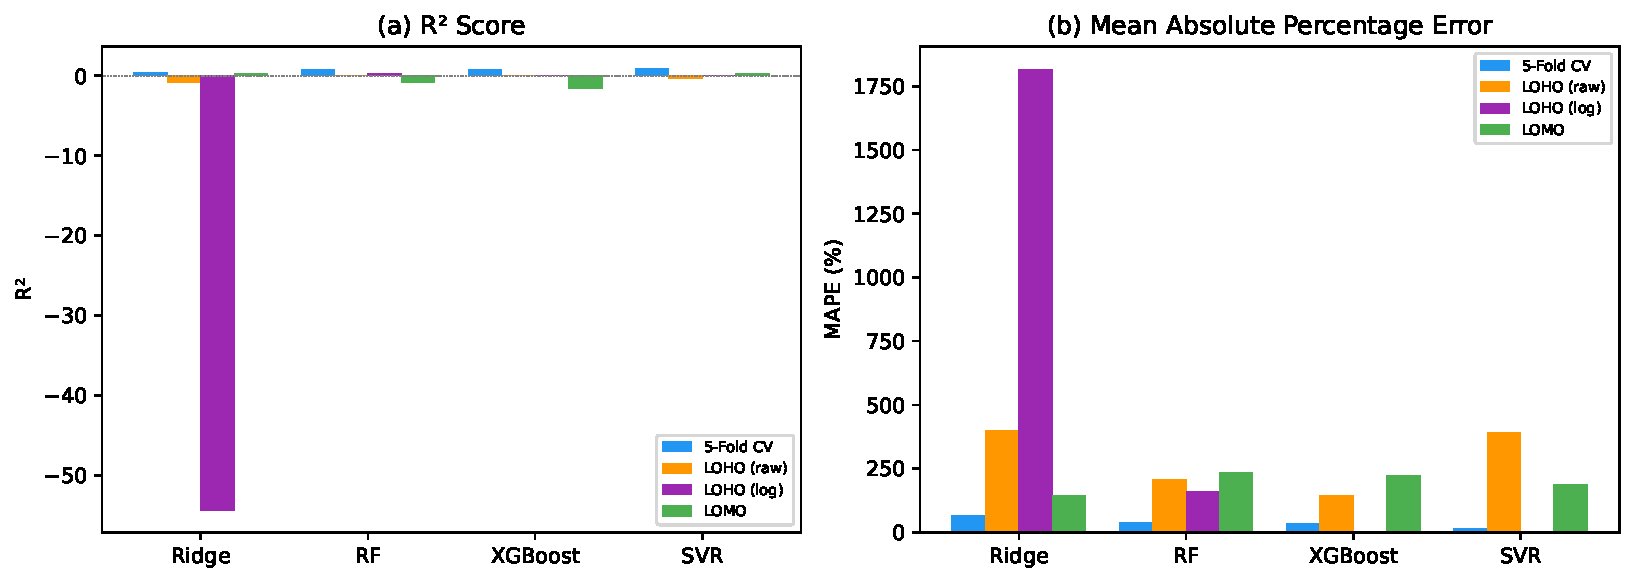
\includegraphics[width=\textwidth]{figures/model_comparison.pdf}
\caption{Comparison of regression methods across evaluation protocols. (a)~$R^2$ score: 5-fold CV yields strong positive values for all methods, while LOHO and LOMO degrade to near-zero or negative. Ridge with log features shows catastrophic degradation under LOHO ($R^2 \approx -55$). (b)~MAPE: 5-fold CV achieves low errors; LOHO errors exceed 1,000\% for Ridge (log). Tree-based methods degrade more gracefully.}
\label{fig:model_comparison}
\end{figure*}

\subsection{Feature Importance via SHAP Analysis}
\label{sec:results_shap}

Fig.~\ref{fig:shap} presents SHAP feature importance decomposed by architecture type.
Three key findings emerge:

\textbf{(1) Overall:} Output complexity, diffusion steps, and model size are the top-three cost drivers, followed by hardware TDP.
Batch size has minimal impact at the scales tested.

\textbf{(2) AR models:} Hardware TDP dominates (mean $|\text{SHAP}| {=}$ \input{results/tex/shap_ar_tdp.tex}\unskip), followed by output complexity (\input{results/tex/shap_ar_complex.tex}\unskip).
AR inference is \emph{hardware-bound}: the platform's power envelope determines total energy more than model architecture.
This aligns with the observation that AR models maintain near-constant power draw during sequential token generation~\cite{samsi2023words}.
This implies that power management strategies (DVFS, power gating) can yield significant energy savings for AR workloads.

\textbf{(3) Diffusion models:} Output complexity (\input{results/tex/shap_diff_complex.tex}\unskip) and diffusion steps (\input{results/tex/shap_diff_steps.tex}\unskip) dominate, with hardware TDP being secondary (\input{results/tex/shap_diff_tdp.tex}\unskip).
Diffusion inference is \emph{workload-bound}: the iterative denoising loop saturates hardware, making workload parameters the dominant cost factors.

This dichotomy has direct implications for system designers: optimizing AR workloads benefits most from hardware power management (lower-TDP platforms save energy proportionally), while diffusion workloads benefit from algorithmic improvements such as step reduction and distillation~\cite{salimans2022progressive}.

\begin{figure*}[t]
\centering
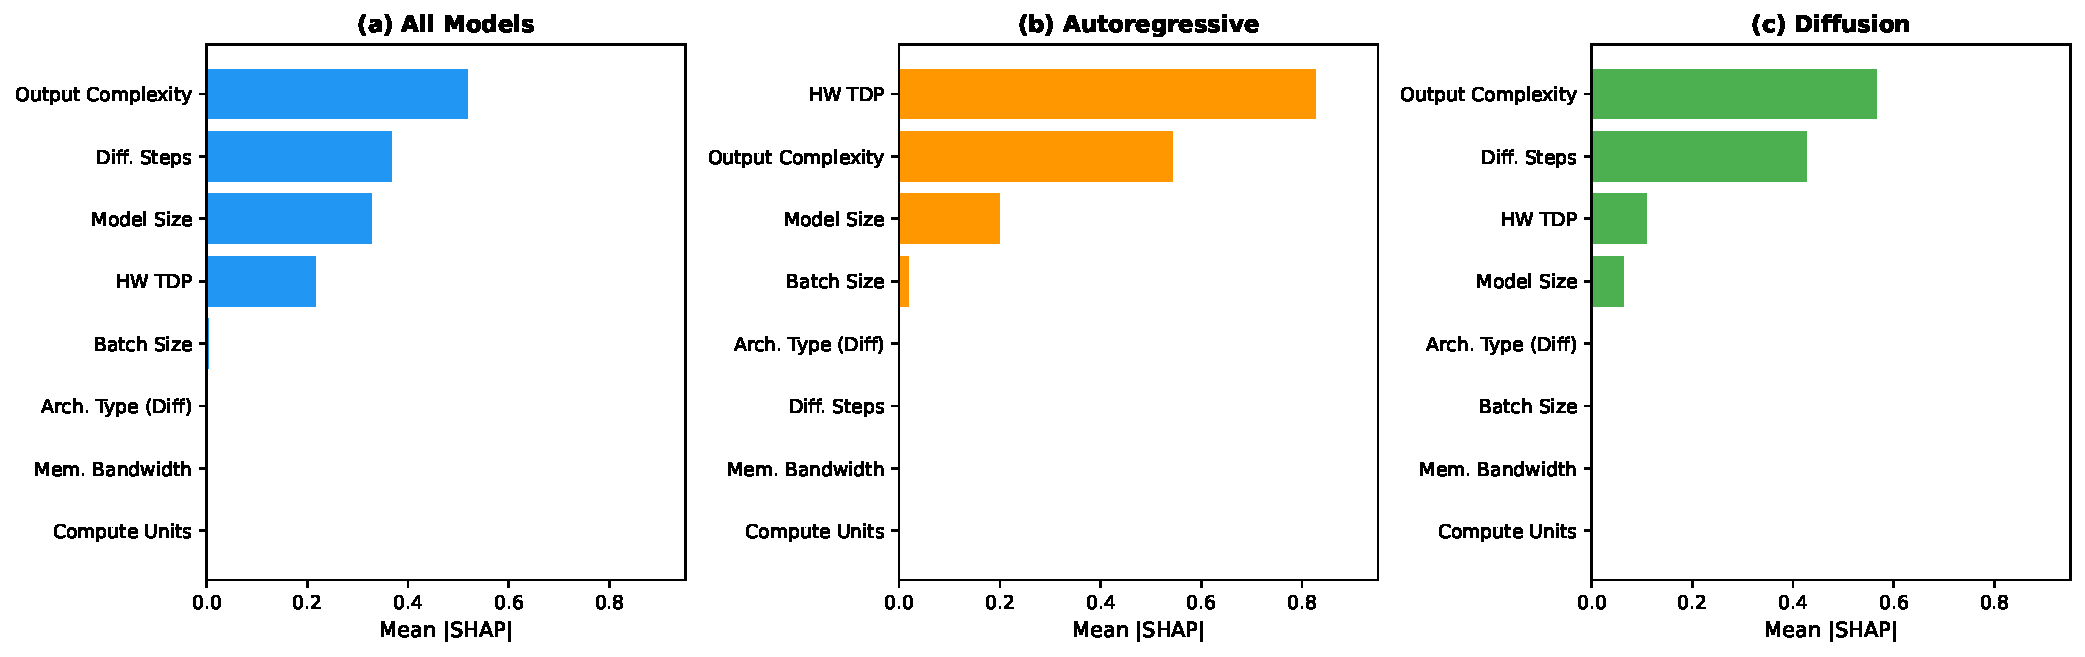
\includegraphics[width=\textwidth]{figures/shap_importance.pdf}
\caption{SHAP feature importance for energy prediction decomposed by architecture type. (a)~All models combined: output complexity, diffusion steps, and model size are the top drivers. (b)~Autoregressive models only: hardware TDP dominates, revealing hardware-bound behavior. (c)~Diffusion models only: output complexity and diffusion steps dominate, revealing workload-bound behavior. All x-axes share the same scale for cross-panel comparison. Features are log-transformed.}
\label{fig:shap}
\end{figure*}

\subsection{Analytical Cost Formula}
\label{sec:results_analytical}

A log-linear analytical model of the form is also fitted:
\begin{equation}
\log(1{+}E) = \beta_0 + \sum_{i=1}^{7} \beta_i \cdot f_i + \beta_8 \cdot \mathbb{1}_{\text{Diff}}
\label{eq:analytical}
\end{equation}
where $f_i$ are log-transformed features and $\mathbb{1}_{\text{Diff}}$ is the architecture indicator.
The fitted coefficients reveal the multiplicative cost structure: energy scales as $E \propto P^{0.46} \cdot C^{0.64} \cdot S^{1.06} \cdot \text{TDP}^{-0.32} \cdot \text{BW}^{-0.95}$, where $P$ is model size, $C$ is output complexity, $S$ is diffusion steps, and the negative TDP/bandwidth exponents reflect that higher-capability hardware completes work faster, reducing energy duration.
This formula achieves $R^2 {=}$\,\input{results/tex/analytical_insample_r2.tex}\unskip{} in-sample and MAPE of \input{results/tex/analytical_loho_mape.tex}\unskip\% under LOHO-CV, confirming that the cross-platform extrapolation challenge persists even with explicitly structured models.
The analytical form is analogous to the roofline model~\cite{williams2009roofline} in spirit---both capture hardware--workload interactions through simple parametric relationships---though the roofline operates on arithmetic intensity while the cost formula operates on high-level specifications.

The negative TDP exponent ($-0.32$) warrants explanation.
Intuitively, higher TDP indicates a more powerful platform that completes inference faster, reducing the time component of energy ($E = P \times t$).
Although the instantaneous power is higher, the reduction in inference time more than compensates, yielding lower total energy.
The negative bandwidth exponent ($-0.95$) reflects a similar effect: higher memory bandwidth reduces data movement bottlenecks, accelerating inference.
The near-unity exponent on diffusion steps ($1.06$) confirms the approximately linear relationship between step count and energy for diffusion models.


%======================================================================
\section{Discussion}
\label{sec:discussion}
%======================================================================

\subsection{The Generalization Gap}
\label{sec:discussion_gap}

The contrast between 5-fold CV ($R^2 {=}$\,\input{results/tex/kfold_best_r2.tex}\unskip) and LOHO-CV ($R^2 {<} 0.1$) constitutes the central finding of this work.
This gap arises from three factors:
(1)~with only three hardware platforms, LOHO-CV evaluates three specific train/test splits rather than a statistically powered sample---the result demonstrates failure on \emph{these} platform pairs but cannot claim generality beyond them;
(2)~the three platforms differ qualitatively (unified vs.\ discrete memory architecture, 17.5$\times$ TDP range, different memory hierarchies), not just quantitatively;
(3)~tree-based models fundamentally cannot extrapolate beyond the range of training data, and with hardware features at the extremes of the training distribution, LOHO prediction becomes extrapolation rather than interpolation.

The asymmetric LOHO performance---where interpolation (A100 held out) succeeds but extrapolation (M4~Pro held out) fails---provides further evidence that the gap is structural.
The A100's specifications fall between the M4~Pro and H100 in terms of TDP, memory bandwidth, and compute units, enabling the regression models to interpolate effectively.
In contrast, the M4~Pro lies outside the convex hull of the training data when it is held out (the remaining platforms are both high-TDP NVIDIA GPUs), forcing extrapolation into an unseen regime.

This finding has important implications for the broader field of hardware cost modeling.
It suggests that simply adding more features or using more expressive models will not bridge the gap; rather, the fundamental challenge is that different hardware architecture classes exhibit qualitatively different energy profiles that cannot be captured by continuous feature interpolation.
Additionally, incomplete model coverage across platforms (Table~\ref{tab:models_hw}) means that LOHO simultaneously tests cross-platform \emph{and} cross-model transfer in some cases, conflating two sources of difficulty.

\subsection{Comparison with Existing Approaches}
\label{sec:discussion_comparison}

Our results can be situated relative to several existing approaches.
NeuralPower~\cite{cai2017neuralpower} achieves high accuracy for CNN power prediction on specific hardware, but does not evaluate cross-platform generalization.
nn-Meter~\cite{zhang2021nnmeter} achieves accurate latency prediction within device families by building device-specific kernel predictors, effectively sidestepping the cross-platform challenge.
HELP~\cite{lee2021help} addresses cross-device prediction through hardware-adaptive transfer, using a small number of measurements on the target device to calibrate.
Our results strongly support the HELP approach: the LOHO failure we observe suggests that some form of target-hardware calibration is essential.

The analytical formula we derive (Eq.~\ref{eq:analytical}) provides a complementary perspective.
Unlike black-box regression, it explicitly captures the multiplicative cost structure and yields interpretable exponents.
However, its LOHO performance (MAPE of \input{results/tex/analytical_loho_mape.tex}\unskip\%) is comparable to the black-box models, confirming that the cross-platform challenge is inherent to the problem rather than an artifact of model choice.
This contrasts with the roofline model~\cite{williams2009roofline}, which provides platform-independent bounds; however, the roofline requires detailed workload characterization (arithmetic intensity) that is not available at the design-time scenario we target.

\subsection{Systems Implications}
\label{sec:discussion_systems}

From a systems design perspective, these results have several practical implications.

First, \emph{hardware-specific calibration is essential}: even ${\sim}$10 profiling runs on the target platform would anchor the model substantially, motivating a ``few-shot hardware adaptation'' workflow.
This aligns with recent trends in transfer learning for hardware modeling~\cite{lee2021help,kaufman2021learned} and suggests that future cost models should be designed with calibration in mind.

Second, the SHAP-identified cost driver dichotomy enables \emph{targeted optimization}: AR workloads benefit from power-efficient hardware selection (since TDP dominates), while diffusion workloads benefit from algorithmic step reduction~\cite{salimans2022progressive}.
For SoC power budgeting, AR inference power can be estimated primarily from TDP, while diffusion inference requires workload characterization.
Integrating these findings with microarchitectural tools (Wattch~\cite{brooks2000wattch}, Accelergy~\cite{wu2019machine}) could enable hierarchical power estimation: rapid top-down system-level estimates with detailed bottom-up validation.

Third, the asymmetric LOHO performance suggests that \emph{hardware architecture class} matters more than individual specifications.
Discrete GPU platforms with CUDA cores and HBM form one class; unified-memory SoCs with integrated GPU cores form another.
Future cost models should incorporate explicit hardware class indicators or employ domain adaptation techniques to bridge the gap between architecture classes.

\subsection{Practical Design Guidelines}
\label{sec:discussion_guidelines}

Based on the analysis, the following guidelines are offered for system designers:
\begin{enumerate}
\item \textbf{Same platform:} If even partial profiling data exists on the target hardware, SVR with log-features provides accurate prediction ($R^2 {>} 0.9$, MAPE ${<} 15$\%) from only eight features.
\item \textbf{Similar platform:} For hardware within the same class (e.g., A100~$\to$~H100), models trained on the source provide reasonable estimates (MAPE ${\sim}$35--60\%).
\item \textbf{Different platform class:} Cross-class prediction (GPU~$\to$~SoC) requires hardware-specific calibration. The analytical formula~\eqref{eq:analytical} provides order-of-magnitude estimates.
\item \textbf{New model architecture:} AR-to-AR and diffusion-to-diffusion transfer is more reliable than cross-paradigm prediction.
\end{enumerate}

\subsection{Limitations}
\label{sec:discussion_limitations}

Several limitations of this study should be acknowledged.

\textbf{Platform diversity:} The three-platform scope limits LOHO generalization assessment.
With $n{=}3$ leave-one-out splits, the results characterize specific platform pairs rather than establishing a general law.
The platforms were selected for architectural diversity, but the resulting LOHO evaluation has limited statistical power.
Expanding to additional platforms (AMD Instinct, Google TPU, Intel Gaudi, FPGA-based accelerators) would strengthen the findings.

\textbf{Dataset size:} The 137 configuration-level data points suffice for the eight-feature models but would not support higher-dimensional approaches or deep learning-based predictors.
The approximately 30 repetitions per configuration provide reasonable variance estimates, but the number of unique configurations is modest compared to studies that profile hundreds of neural architectures~\cite{zhang2021nnmeter}.

\textbf{Incomplete coverage:} Not all models were tested on all platforms (Table~\ref{tab:coverage}), introducing asymmetry in cross-validation evaluation.
This means that LOHO performance for a given held-out platform depends not only on the platform gap but also on which models are available for training and testing.

\textbf{Model selection:} The seven generative models, while spanning both AR and diffusion paradigms across four modalities, do not cover the full landscape of generative AI.
Notably absent are decoder-only LLMs at the 70B+ scale, text-to-video models beyond AnimateDiff, and multimodal models that combine text and image generation.
Results may not generalize to these architectures.

\textbf{Quantization and optimization:} All models were evaluated in their default precision (typically FP16 or BF16) without quantization, pruning, or other optimization techniques.
Quantized models (INT8, INT4) may exhibit different energy scaling relationships, and specialized inference engines (TensorRT, vLLM) may alter the hardware utilization patterns.

\textbf{Measurement methodology:} The instrumentation approaches differ across platforms (\texttt{nvidia-smi} for GPUs, \texttt{powermetrics} for M4~Pro), introducing potential systematic differences in what is measured.
While both capture system-level inference energy, the granularity and scope of power measurement are not identical.

\subsection{Threats to Validity}
\label{sec:threats}

\textbf{Internal validity:}
The primary threat is potential data leakage across cross-validation folds.
We mitigate this by aggregating repeated measurements to configuration-level means before splitting, ensuring that repetitions of the same configuration never appear in both training and test sets.
Hyperparameters were set to standard defaults without tuning on evaluation data, reducing the risk of overfitting to the specific cross-validation splits.

\textbf{External validity:}
The three-platform, seven-model scope limits the generalizability of specific numerical results (e.g., the exact $R^2$ values).
However, the qualitative finding---that cross-platform prediction is fundamentally harder than within-platform prediction---is likely to hold more broadly, as it is grounded in the structural difference between hardware architecture classes rather than idiosyncratic features of specific platforms.

\textbf{Construct validity:}
We use system-level energy as the primary cost metric, which includes both the inference workload and background system activity.
While this is the relevant quantity for operational cost estimation, it may introduce noise from unrelated system processes.
The approximately 30 repetitions per configuration help average out such noise.


%======================================================================
\section{Conclusion}
\label{sec:conclusion}
%======================================================================

This paper has presented a predictive cost modeling framework for generative AI inference across heterogeneous hardware.
The key findings are threefold:
(1)~within-platform prediction is accurate ($R^2 {=}$\,\input{results/tex/kfold_best_r2.tex}\unskip, MAPE ${\approx}$\,\input{results/tex/kfold_best_mape.tex}\unskip\%), validating that feature-based cost modeling captures the essential structure of inference energy;
(2)~cross-platform prediction via LOHO-CV reveals a substantial generalization gap ($R^2 {<} 0.1$), demonstrating that training on a small number of platforms is insufficient for reliable extrapolation---a critical insight for the research community seeking universal cost models;
(3)~SHAP analysis uncovers a hardware-bound vs.\ workload-bound dichotomy between AR and diffusion architectures, providing architecture-specific optimization guidance.

For system designers and practitioners, these results suggest combining general-purpose models with lightweight hardware-specific calibration: power management for AR workloads, step reduction for diffusion workloads.
The analytical cost formula (Eq.~\ref{eq:analytical}) provides interpretable, design-time estimates when detailed profiling is unavailable, while the SHAP decomposition guides where to focus optimization effort.

The generalization gap identified in this work is not merely a modeling failure---it reflects a fundamental challenge in cross-platform performance prediction that has implications beyond generative AI.
As hardware architectures diversify (GPUs, SoCs, NPUs, FPGAs), the assumption that a model trained on one platform class can predict behavior on another becomes increasingly tenuous.
Addressing this challenge will require either richer hardware descriptors that capture architectural differences beyond TDP and core counts, or few-shot adaptation techniques that leverage a small number of target-platform measurements.

Future work should expand the platform coverage to include FPGAs, NPUs, and quantized model variants, and apply transfer learning or meta-learning for few-shot hardware adaptation.
Additionally, incorporating dynamic features such as memory utilization patterns and thermal throttling behavior may help bridge the cross-platform gap.
The framework presented here provides a foundation for these extensions and a benchmark against which future cross-platform cost models can be evaluated.

\section*{CRediT Authorship Contribution Statement}

\textbf{Yongjun Kim:} Conceptualization, Methodology, Software, Validation, Formal analysis, Investigation, Data curation, Writing -- original draft, Writing -- review \& editing, Visualization.

\section*{Declaration of Competing Interest}

The author declares that there is no known competing financial interests or personal relationships that could have appeared to influence the work reported in this paper.

\section*{Data Availability}

The measurement data and analysis code are available from the author upon reasonable request.

\section*{Acknowledgments}

This work was supported by Ajou University.

\bibliographystyle{elsarticle-num}
\bibliography{refs}

\end{document}
